\chapter{Cơ sở lý thuyết}

% 2.1
\section{Tổng quan Hệ thống tư vấn}

\subsection{Cách để tham chiếu tới hình ảnh}
Để tham chiéu tới hình vẽ ta thực hiện như sau: \textbf{ \autoref{fig:overview-recsys}}.

\begin{figure}
    \centering
    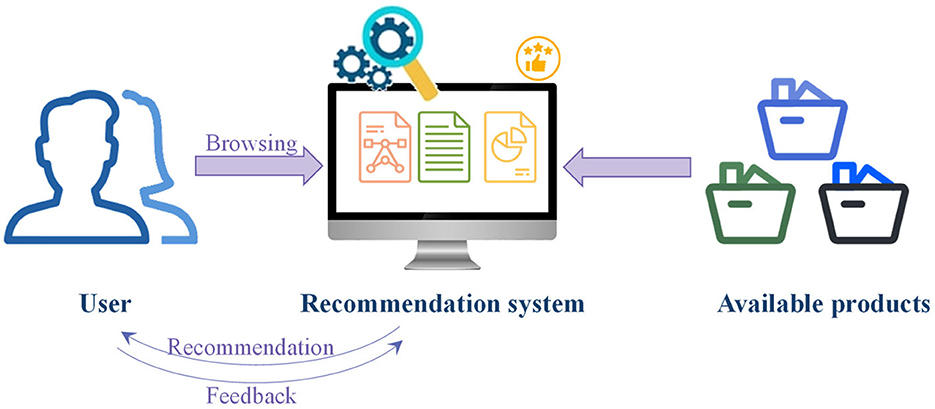
\includegraphics[width=0.7\linewidth]{images/overview_recsys.jpg}
    \caption{Tổng quan Hệ thống tư vấn}
    \label{fig:overview-recsys}
\end{figure}


\subsection{Cách để tham chiếu và vẽ bảng}

Tham chiếu đến bảng: \textbf{\autoref{tab:ranking_comparison}}so sánh hiệu suất đánh giá của mô hình.

\begin{table}[h!]
    \centering
    \caption{So sánh hiệu quả giữa các phương pháp đề xuất xếp hạng.}
    \label{tab:ranking_comparison}
    \begin{tabular}{lcc}
        \toprule
        \textbf{Độ đo} & \textbf{Lọc dựa trên nội dung} & \textbf{Đề xuất dựa trên độ phổ biến} \\
        \midrule
        \textbf{NDCG@10}  & \textbf{0.230} & 0.089 \\
        \textbf{Recall@10} & \textbf{0.171} & 0.149 \\
        \textbf{MRR@10}    & \textbf{0.062} & 0.053 \\
        \textbf{Precision@10}& \textbf{0.017} & 0.015 \\
        \bottomrule
    \end{tabular}
\end{table}